\lecture{Análise léxica usando {\tt flex}}
\frame{\title{\insertlecture}\maketitle}

\section{Análise léxica usando {\tt flex}}

\frame{\tableofcontents}

\subsection{Histórico}

\begin{frame}{História e princípios}
  \begin{itemize}
  \item{\color{gray!70!black}\href{https://www.gnu.org/software/bison/}{\tt
      bison} descende do
    \href{(https://pt.wikipedia.org/wiki/Yacc}{\tt yacc} desenvolvido
    por
    \href{https://en.wikipedia.org/wiki/Stephen_C._Johnson}{Stephen
      C. Johnson} entre 1975 e 1978 no
    \href{https://pt.wikipedia.org/wiki/Bell_Labs}{Bell Labs}.}
  \item Johnson trabalhou em estreita colaboração com
    \href{https://en.wikipedia.org/wiki/Alfred_Aho}{Alfred Aho}
    e sob a base teórica sólida do trabalho de
    \href{https://www-cs-faculty.stanford.edu/~knuth/}{Don E. Knuth}
    na área de compiladores.
  \item Uma das motivações era desenvolver extensões para o
    programa \href{https://en.wikipedia.org/wiki/Troff}{\tt troff}
    usando a {\bf filosofia
    \href{https://en.wikipedia.org/wiki/Unix_philosophy}{Unix}}.
  \item \alert{\tt flex} descende do \alert{\tt lex} desenvolvido por
    \href{https://en.wikipedia.org/wiki/Mike_Lesk}{Mike Lesk}
    e \href{https://en.wikipedia.org/wiki/Eric_Schmidt}{Eric Schmidt}
    em 1975 no Bell Labs.
  \end{itemize}
\end{frame}

\subsection{Terminologia}

\begin{frame}{Terminologia}
  \begin{tabular}[h]{lcl}
    \alert{\it token\/}& -- & símbolo terminal\\
    lexema & -- &cadeia de caracteres \\
    padrão & -- &conjunto de lexemas que representam um {\it token\/}
  \end{tabular}\bigskip

  \pause\small
  Exemplo: {\tt printf("Total=\%d", valor);}\\
  Os lexemas {\tt printf} e {\tt valor} combinam com o padrão para
  o {\it token\/} {\bf id} (identificador) e o lexema {\tt "Total=\%d"}
  combina com o {\it token\/} {\bf literal}.\\

  \pause\bigskip
  \begingroup
  \footnotesize\center
  \begin{tabular}[h]{lll}\toprule
    {\sc\it token\/}& \sc descrição informal do padrão & \sc lexema(s)\\
    \midrule
    {\bf if} & caracteres {\tt 'i'} e {\tt 'f'} & if \\
    {\bf else} & caracteres {\tt 'e'}, {\tt 'l'}, {\tt 's'}, {\tt 'e'}  & else \\
    {\bf relop} & {\tt >} ou {\tt <} ou {\tt >=} ou {\tt <=} ou {\tt !=}
                  ou {\tt ==} & >, <, >=, <=, !=, == \\
    {\bf id} & letra seguida por letras e dígitos & valor, printf, x, i \\
    {\bf num} & qualquer constante numérica & 3.14, 5, .7 \\
    {\bf literal} & quaisquer caracteres entre ``s & {\tt "Valor \%d"} \\
    \bottomrule
  \end{tabular}
  \endgroup
  \bigskip

    \scriptsize
    Observação: quando padrões coincidem, mais informações devem
    ser repassadas adiante.
\end{frame}


\begin{frame}{Terminologia, cont.}

  \hfil padrão $\rightarrow$ \alert{expressão regular} --
  linguagem ``padrão'' dos analisadores léxicos\\\bigskip

  expressão regular $\rightarrow$ implementação requer simulação de um
  \alert{autômato finito determinístico}~(AFD)

  \note{Mesmo nos analisadores implementados manualmente, o
    uso de AFD ajuda a lidar com a complexidade e correção do
  código de análise dos padrões.}
\end{frame}

\subsection{Analisador léxico}

\begin{frame}{Analisador léxico}{Função}

  Primeira fase de compilação:

  \begin{enumerate}
  \item Lê a entrada de caracteres do código-fonte;
  \item Agrupa-os em lexemas;
  \item Produz uma saída de sequência {\it tokens\/} para cada lexema;
  \item O fluxo de {\it tokens\/} é enviado para o analisador
    sintático ({\it parser\/}).
  \end{enumerate}\bigskip

  Nesta fase, o analisador léxico pode interagir com a tabela
  de símbolos.
\end{frame}


\begin{frame}{Vantagens da separação do analisador sintático}

\pause

\begin{itemize}
\item Simplicidade do projeto do compilador.
\item Melhoria na eficiência.
\item Portabilidade.
\end{itemize}

\end{frame}

\subsection{Expressões regulares}
\frame{\tableofcontents[currentsubsection]}

\begin{frame}{Regras - expressões regulares}

 Caracteres especiais:\bigskip

 \footnotesize
 \center
\begin{tabular}{ll}\toprule
  \bf expressão  & \bf  descrição do padrão \\
  \midrule
  {\tt .}          &  combina com qualquer caracter, com exceção do '{$\backslash$n}'\\
  {\tt []}         &  classe de caracteres: combina com qualquer\\
                 &  caracter dentro do colchetes\\
   \^{}            &  combina a expressão regular que o segue no\\
                 &  início da linha\\
  {\tt \$}          &  combina a expressão regular que o precede no\\
                 &  início da linha\\
  {\tt \{\}}         &  especifica o número mínimo e máximo de vezes\\
                 &  que a expressão que o precede pode combinar\\
  {\tt *}          &  combina com {\bf zero} ou mais cópias da expressão\\
                 &  que o precede pode combinar\\
  {\tt +}          &  combina com {\bf uma} ou mais cópias da expressão\\
                 &  que o precede pode combinar\\
  {\tt ?}          &  combina com zero ou uma cópia da expressão\\
                 &  que o precede pode combinar\\
  \bottomrule
\end{tabular}
\end{frame}

\begin{frame}{Regras - expressões regulares (cont.)}

 Caracteres especiais:\bigskip

 \footnotesize
 \center
 \begin{tabular}{ll}
   \toprule
   \bf expressão &\bf    descrição do padrão\\
   \midrule
   {\tt $\backslash$}   & usado para mudar a classe dos caracteres especiais,\\
               & por exemplo, {\tt $\backslash$*} combina com o caracter asterisco\\
    {\tt |}         &   operador de alternância\\
    {\tt "..."}     &   a expressão dentro das aspas é tratada literalmente\\
    {\tt ()}       &    agrupa um conjunto de expressões\\
    {\tt /}        &    combina somente se a expressão antes e depois\\
                 &da barra combinarem\\
   \bottomrule
 \end{tabular}
 \end{frame}

\begin{frame}{Exemplo - expressões regulares}

 \footnotesize
 \center
 \begin{tabular}{ll}
   \toprule
   \bf expressão & \bf          descrição do padrão\\
   \midrule
   {\tt .+}      &           combina com qualquer caracter\\
   {\tt [a-zA-Z]+} &         combina com qualquer conjunto de letras\\
                 &    maiúsculas ou minúsculas - {\tt abc}, {\tt AbC}, {\tt zZz}\\
   {\tt [0-9]+}      &       combina com qualquer sequência de números -\\
                 &  {\tt 0}, {\tt 12}, {\tt 5633}, {\tt 1111}\\
   {\tt -?[0-9]}        &     combina com número inteiro precedido ou não\\
                 & por um sinal {\tt -}\\
   {\tt a(bc|de)}      &     combina com {\tt abc} ou {\tt ade}\\
   {\tt 0/1}            &    combina com {\tt 0} na string {\tt 01} mas não {\tt 0} ou {\tt 02}\\
   {\tt b\{1,4\}}          &   combina de 1 a 4 ocorrências da letra {\tt b}\\
   {\tt 2\{5\}}            &   combina com 5 ocorrências do número {\tt 2}\\
   {\tt [ $\backslash$t]*} &   combina opcionalmente espaços e tabulações\\
   \^{}{\tt a|o\$}          &    combina linhas que contenham strings\\
                 & onde a primeira letra seja 'a' ou a última letra seja 'o'\\
                 & - "{\tt andar$\backslash$n}", "{\tt mercado pago$\backslash$n}", "\sout{{\tt sem novidade$\backslash$n}}"\\
   \bottomrule
 \end{tabular}
\end{frame}

\begin{frame}{Expressão regular}{Autômato finito}

\begin{itemize}
  \item Operadores ``{\tt <=}'' e ``{\tt <}''\\ 
\end{itemize}

\usetikzlibrary{arrows.meta,automata,positioning}
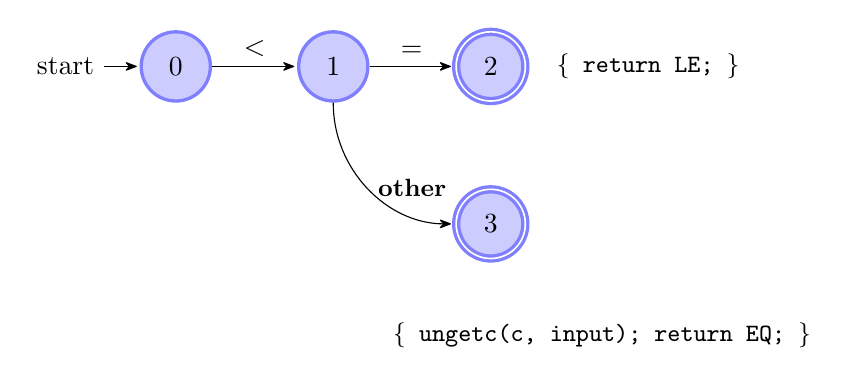
\begin{tikzpicture}[shorten >=1pt,node distance=2cm,on grid,>={Stealth[round]},
every state/.style={draw=blue!50,very thick,fill=blue!20},bend angle=45]
\node[state,initial] (q0) {$0$};
\node[state] (q1) [right=of q0] {$1$};
\node[state,accepting] (q2) [right=of q1] {$2$};
\node[state,accepting] (q3) [below=of q2] {$3$};
%% Returns.
\node [right=of q2] {\small\tt \{ return LE; \}};
\node [below right=of q3] {\small\tt \{ ungetc(c, input); return EQ; \}};
%% Paths.
\path[->] 
    (q0) edge node [above] {$<$} (q1)
    (q1) edge node [above] {$=$} (q2)
    (q1) edge [bend right] node [above,right] {\bf\small other} (q3)
;
\end{tikzpicture}

\end{frame}

\begin{frame}[fragile]{Expressão regular}{Autômato finito, cont.}

  Reconhecimento de Palavras-chave e identificadores

\end{frame}


\subsection{Usando {\tt flex}}
\frame{\tableofcontents[currentsubsection]}

\begin{frame}{Criando um analisador léxico}

\includegraphics[scale=.4]{lex-compilador.png}
\end{frame}

\begin{frame}{Fluxo de compilação}
  \center\footnotesize
  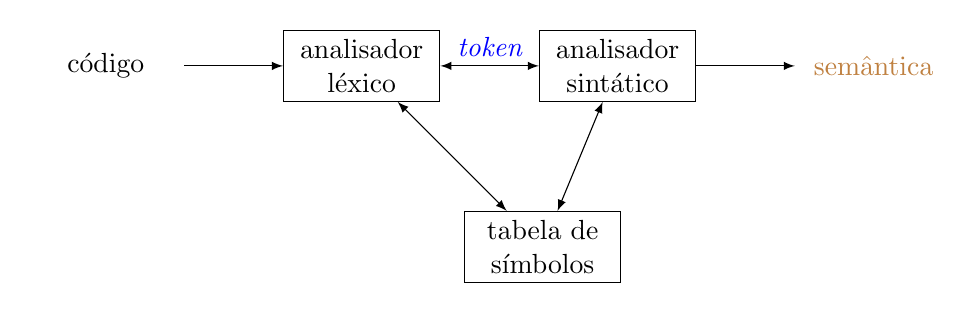
\begin{tikzpicture}
    [text width=1.75cm,align=center,node distance=3.25cm,>=latex]
    \node (input) {código};
    \node[draw] (lex) [right of=input] {analisador léxico};
    \node[draw] (yacc) [right of=lex] {analisador sintático};
    \node[draw] (table) [below right of=lex] {tabela de símbolos};
    \node[] (func) [right of=yacc] {\color{brown}semântica};
    \path (input) edge[->] (lex);
    \path (lex) edge[<->] node[above] {\color{blue}\it token} (yacc);
    \path (yacc) edge[->] (func);
    \path (lex) edge[<->] (table);
    \path (yacc) edge[<->] (table);
  \end{tikzpicture}
\end{frame}

\begin{frame}[fragile]{Seções do arquivo}
\begin{lstlisting}[language=C,frame=single]
definições

%%

regras na forma

Padrão (expressão regular)     {Ação (código C)}

%%

funções auxiliares (código C)

\end{lstlisting}
\end{frame}

\begin{frame}[fragile]{Fluxo de compilação}
\begin{lstlisting}[language=bash]
$ lex -o arquivo.yy.c arquivo.l
$ gcc -o arquivo.exe arquivo.yy.c
\end{lstlisting}\bigskip

\pause Variáveis e funções internas

 \center\small
 \begin{tabular}{ll}
   \toprule
   \bf variável global $\qquad$&  \bf descrição\\
   \bf ou função   & \\
   \midrule
   {\tt yylex()}  &  realiza leitura dos caracteres de entrada        \\
   {\tt yyin}     &  deve receber o ponteiro para o arquivo a ser lido \\
   {\tt yyval}    & usada para passar o valor do {\it token\/} para o {\it parser\/}\\
   \bottomrule
 \end{tabular}
\end{frame}

\subsection{Exemplo}
\frame{\tableofcontents[currentsubsection]}

\begin{frame}{Exemplo - especificação flex}{$\mu$C}
  \center
  \begin{tabular}{rrl}
    {\bf if} & $\rightarrow$ & {\tt if} \\
    {\bf else} & $\rightarrow$ & {\tt else} \\
    {\bf relop} & $\rightarrow$ & {\tt <} | {\tt <=} | {\tt >} | {\tt >=} | {\tt =} | {\tt !=} \\
    {\bf id}    & $\rightarrow$ & {\bf letra}({\bf letra}|{\bf dígito})* \\
    {\bf num}    & $\rightarrow$ & {\bf dígito}+(.{\bf dígito})? \\
   \end{tabular}
 \end{frame}

\begin{frame}{Exemplo - especificação flex, cont.}{$\mu$C}
  \small
  \center
  \begin{tabular}{c|c|c}
    \toprule
    \bf\color{blue} expressão regular
    &\bf\color{blue}  token
    &\bf\color{blue} valor de atributo \\
    \midrule
    {\bf ws} &  --      & -- \\
    {\tt if}   & {\tt IF}  & -- \\
    {\tt else}   & {\tt ELSE}  & -- \\
    {\bf id}   & {\tt ID}  & ponteiro para entrada na tabela \\
    {\bf num}   & {\tt NUM}  & ponteiro para entrada na tabela \\
    {\tt <}   & {\tt RELOP} & {\tt LT} \\
    {\tt <=}   & {\tt RELOP} & {\tt LE} \\
    {\tt >}   & {\tt RELOP} & {\tt GT} \\
    {\tt >=}   & {\tt RELOP} & {\tt GE} \\
    {\tt =}   & {\tt RELOP} & {\tt EQ} \\
    {\tt !=}   & {\tt RELOP} & {\tt NE} \\
    \bottomrule
   \end{tabular}
 \end{frame}

\begin{frame}[fragile]{Exemplo - código}
 \tiny
\begin{lstlisting}
%{ /* declarações de constantes */
    ID, IF, THEN, ELSE, GE, GT, LE, LT, EQ, NE, NUM, RELOP
%}
 /* definições regulares - regras de tradução */
ws                   [ \t\n]+
letter               [A-Za-z_]
digit                [0-9]
id                   {letter}({letter}|{digit})*
num                  {digit}+(\. {digit}+)?
%%
{ws}                { /* espaço em branco, nada é retornado ao parser */ }
if                  {return IF;}
then                {return THEN;}
else                {return ELSE;}
{id}                {yyval = install_id(); return ID;}
{num}               {yyval = install_num(); return NUM;}
"<"                 {yyval = LT; return RELOP;}
"<="                {yyval = LE; return RELOP;}
">"                 {yyval = GT; return RELOP;}
">="                {yyval = GE; return RELOP;}
"="                 {yyval = EQ; return RELOP;}
"!="                {yyval = NE; return RELOP;}
%%
/* procedimentos auxiliares */
install_id() { ... }
install_num() { ... }
main() { /* procedimento principal */
  yyin = fopen(argv[1], "r");
  yylex();
}
\end{lstlisting}
\end{frame}

\begin{frame}{Exemplo - observações}
  \begin{itemize}
  \item Ambiguidades de cadeias com mesmo prefixo são solucionadas
    usando \alert{regra da sequência mais longa}. Exemplo: {\tt >} e
    {\tt >=}.  \pause
  \item A palavra-chave {\tt if} \alert{precede} o padrão {\bf id}.
    Portanto não será possível usar um identificador ``if''.
    Palavras-chave comumente são reservadas nas linguagens atuais.
    \pause
  \item O procedimento {\tt install\_num()} deve \alert{converter} o
    lexema para o tipo de dados esperado para o número ({\tt int},
    {\tt float}, $\ldots$).  \pause
  \item O procedimento {\tt install\_id()} deve manipular o lexema
    na \alert{tabela de símbolos}.
  \end{itemize}
\end{frame}

\subsection*{Referências}

\begin{frame}{Referências}

  \begin{itemize}
  \item Alfred V. Aho, Monica S. Lam, Ravi Sethi, Jeffrey D. Ullman.
    Compiladores: Princípios, Técnicas e Ferramentas. Editora
    Pearson, 2$^a$ edição, 2007.
  \item David Hanson, Christopher
    Fraser. \href{https://www.amazon.com.br/Retargetable-Compiler-Design-Implementation/dp/0805316701}{A
      Retargetable C Compiler: Design and Implementation}. Editora
    Addison-Wesley, 1995.

  \item John
   Levine. \href{https://www.oreilly.com/library/view/flex-bison/9780596805418/}{flex \& bison}. Editora O'Reilly, 2009.

  \item {\tt Flex} home page {\tt http://www.gnu.org/software/flex/}, Free
    Software Foundation.
  \end{itemize}
 \end{frame}
